\chapter{Lecture nine: Component Design and Model Component}
\section{Component design}
\subsection{Results}
The results are a description of the system's components, typically in a UML diagram, more-so a specification of each major part. There are details of individual components included. Connections between components. This is, furthermore, an iterate architecture, namely use and revise division into components.

\begin{figure}[H]
    \centering
    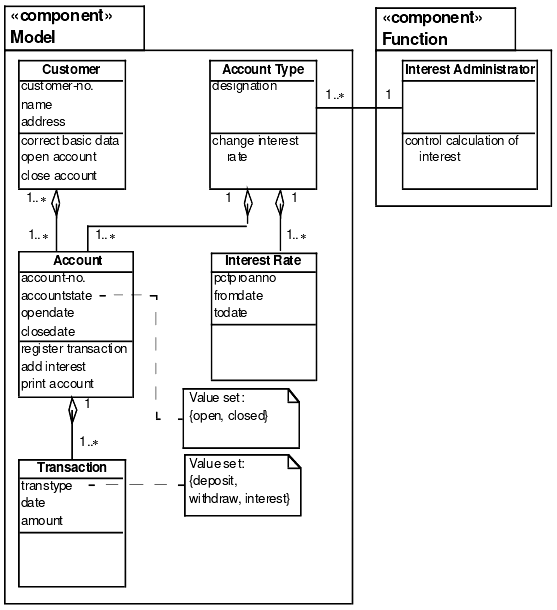
\includegraphics[width=0.5\textwidth]{figures/componentdesignresults.png}
\end{figure}

\subsection{Key concepts: From architecture to components}
\begin{center}
    Respect the component architecture \\
    Adapt component designs to the technical possibilities
\end{center}
\begin{figure}[H]
    \centering
    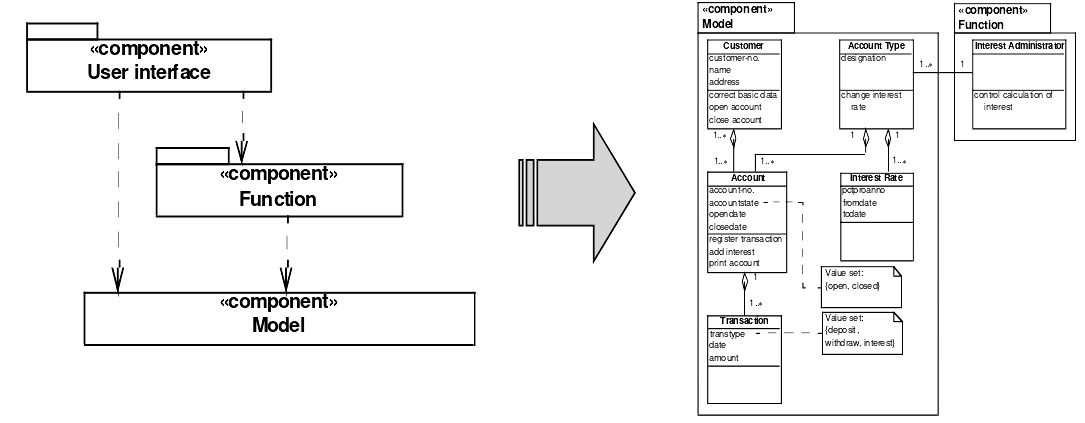
\includegraphics[width=0.8\textwidth]{figures/componentdesignfromarchtocomponents.png}
\end{figure}

\subsection{Activities}
Design \textbf{model and function} components and \textbf{connect} these components.
\begin{figure}[H]
    \centering
    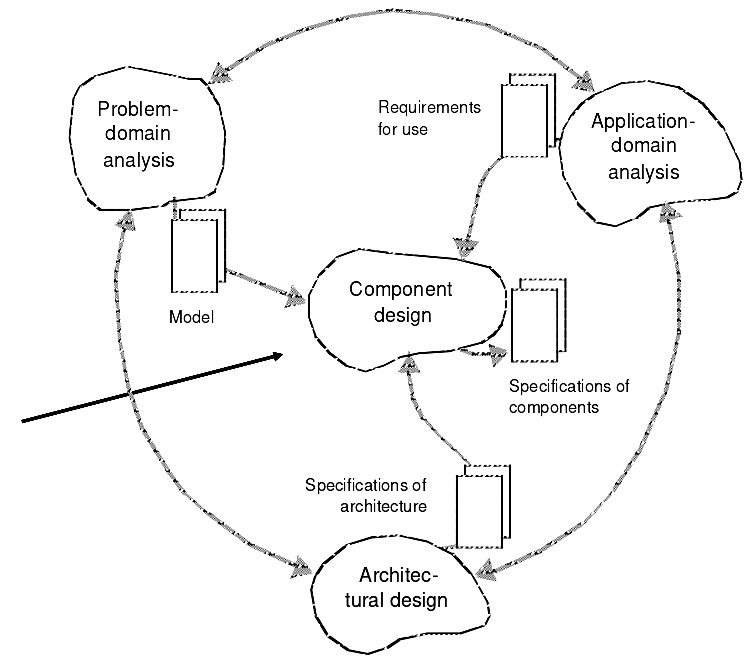
\includegraphics[width=0.5\textwidth]{figures/componentdesignactivities.png}
\end{figure}

\begin{table}[H]
\centering
\resizebox{\textwidth}{!}{%
\begin{tabular}{lll}
\hline
\textbf{Activity}              & \textbf{Content}                                                & \textbf{Concepts}                         \\
\hline
Model component       & How is the model represented as classes in the system? & Model component and attribute    \\
Function component    & How are the functions implemented?                     & Function component and operation \\
Connecting components & How are components connected?                          & Component and connection        \\
\hline
\end{tabular}%
}
\end{table}

\subsection{Summary}
\begin{figure}[H]
    \centering
    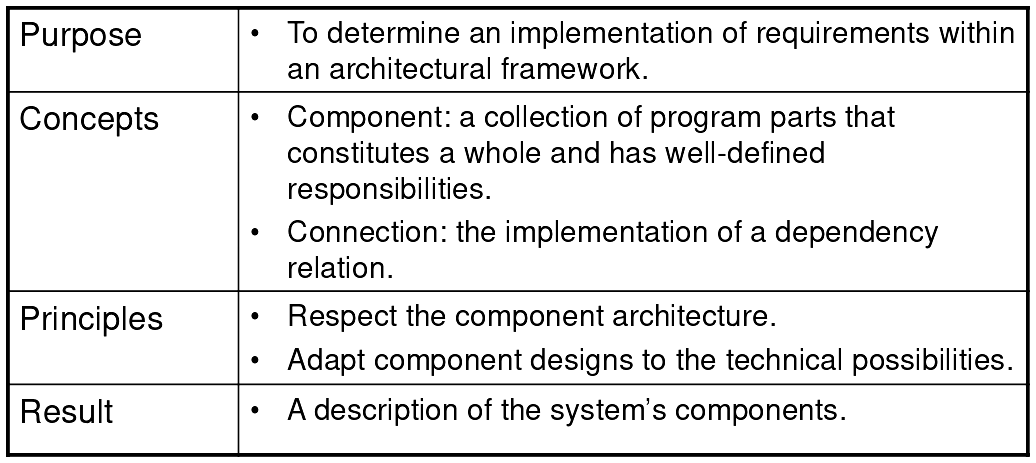
\includegraphics[width=0.7\textwidth]{figures/componentdesignsummary.png}
\end{figure}

\section{Model components}
\subsection{Results}
The point of departure is the class diagram from the \textbf{problem domain analysis}. Extend with representation of behaviour described in the \textbf{statechart diagrams}.
The result of the model-component activity is a revised version of the class diagram from the previous analysis activity. These revisions could typically entail additional classes, attributes, and structures to represent events. Figure shows a revised class diagram from the figure shown in section \ref{modelcomponents:bankexample}.

\begin{figure}[H]
    \centering
    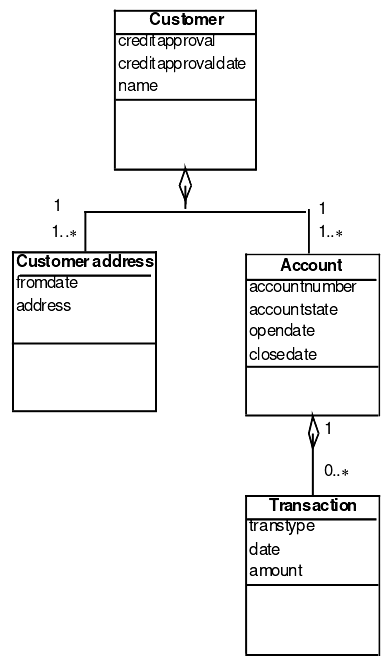
\includegraphics[width=0.35\textwidth]{figures/modelcomponentresults.png}
\end{figure}

\subsection{Key concept: From totality to part}
\textbf{Component:} A collection of program parts that constitutes a whole and has well-defined responsibilities. \textbf{Responsibility of the model component:} Maintain an updated representation of the problem domain.

\begin{figure}[H]
    \centering
    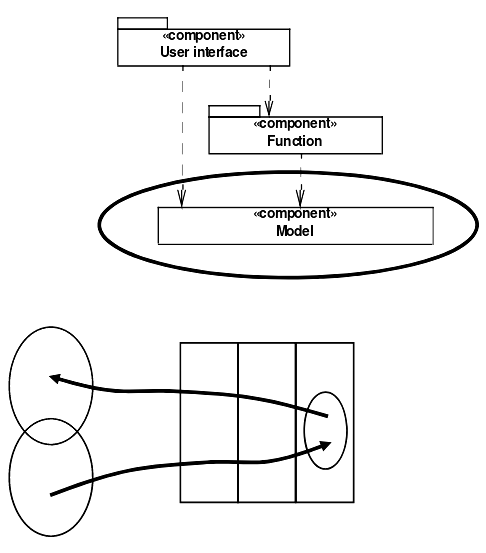
\includegraphics[width=0.5\textwidth]{figures/modelcomponentfromtotalitytopart.png}
\end{figure}

\subsection{Activities}
You start by examining the class diagram and the statechart diagrams from the \textbf{problem-domain} model produced in the analysis activity, and you represent private events and their attributes.
Next, you look at alternative ways of representing common events. Finally, consider restructuring the classes to obtain a simpler and more efficient model component. You thus extend the existing class diagram with new classes, attributes, and structures.

\begin{figure}[H]
    \centering
    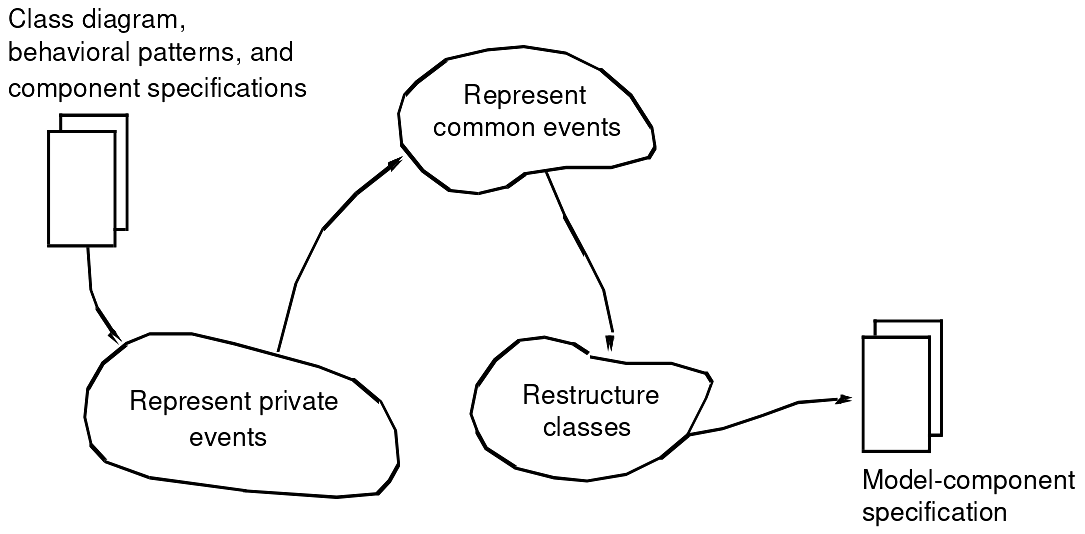
\includegraphics[width=0.7\textwidth]{figures/modelcomponentactivities.png}
\end{figure}

\subsection{Example of a bank system}\label{modelcomponents:bankexample}
This figure shows an example of the starting point of the model component activity, consisting of \textbf{a class diagram, statechart diagrams, and an event table}.
\begin{figure}[H]
    \centering
    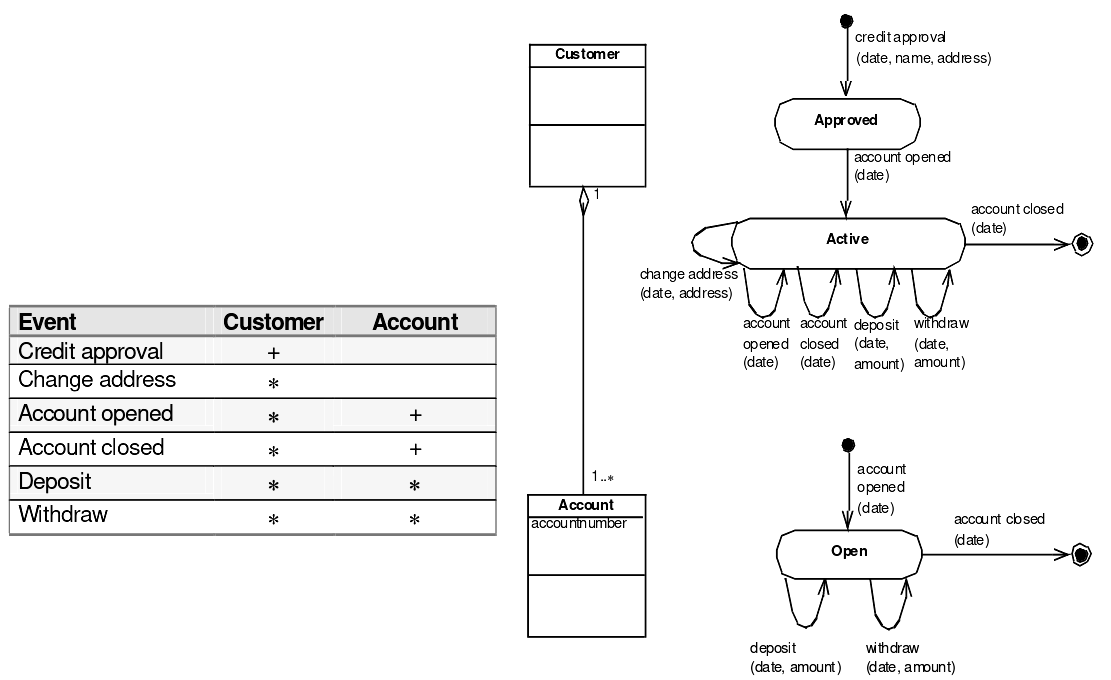
\includegraphics[width=\textwidth]{figures/modelcomponentbankexample.png}
\end{figure}

\subsection{Represent private events}
Private events are events that involve only one problem-domain object. An event table is useful for identifying these private events. Representing private events is straightforward. Events that happen at most once can be represented by class attributes. An event that occurs an arbitrary number of times requires a new class.

\noindent General guidelines:
\begin{itemize}
    \item Events that only occur in sequence and selection:
    \begin{itemize}
        \item Represent these events as a state attribute in the class described by the statechart diagram. 
        \item Every time one of the involved events occurs, the system shall assign a new value to the state attribute.
        \item Integrate the attributes of the involved events in to the class.
    \end{itemize}
    \item Events that occur in iterations:
    \begin{itemize}
        \item Represent these events as a new class; attach them to the class described by the statechart diagram using an aggregation structure. 
        \item For each iteration, the system shall generate a new object from the class.
        \item Integrate the event attributes into the new class.
    \end{itemize}
\end{itemize}

The event \texttt{change address} is private to the class Customer, as seen on previous figures. It is an iteration in the statechart diagram of the class. Represent this event as a new class, as seen on this figure.

The event \texttt{credit approval} is private to the class Customer. It is part of a sequence in the statechart diagram. Represent this event as an attribute, as shown in this figure.

\begin{figure}[H]
    \centering
    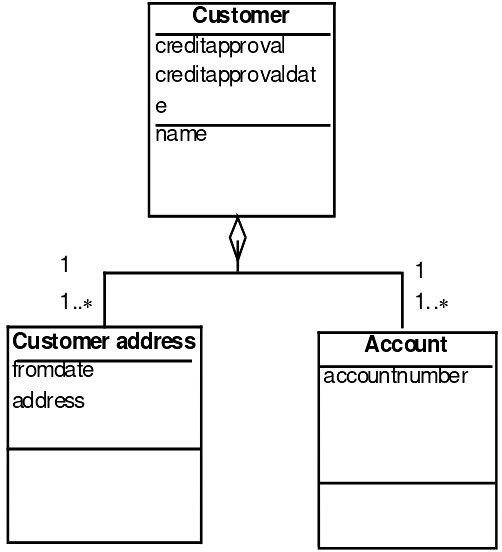
\includegraphics[width=0.35\textwidth]{figures/modelcomponentprivateevents.png}
\end{figure}

Note that in practice you would have to include other criteria like time, space, and security.

\subsection{Represent common events}
If the given event is involved in the statechart diagrams in different ways, represent it in relation to the class that offers the simplest representation. 

If the event is involved in the statechart diagrams in the same way, you must weigh possible representations against each other.

\subsubsection{Solution A}
The events \texttt{deposit} and \texttt{withdraw} are iterations in both the Customer and Account classes.One option is to represent these events as new classes under Account.

\begin{figure}[H]
    \centering
    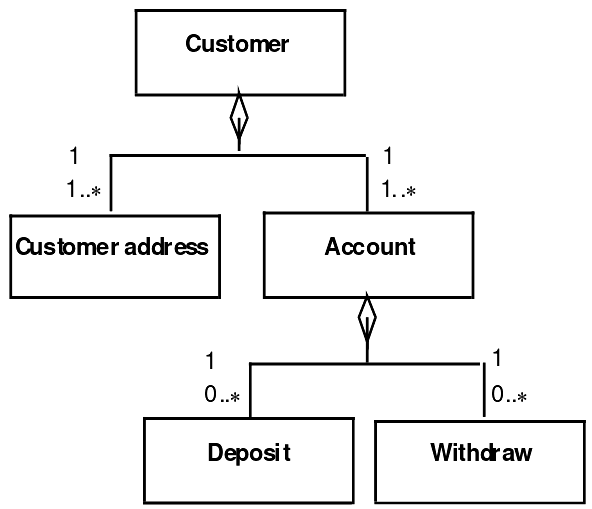
\includegraphics[width=0.35\textwidth]{figures/modelcomponentsolutiona.png}
\end{figure}

\subsubsection{Solution B}
Alternatively, the events \texttt{deposit} and \texttt{withdraw} can be represented as new classes under Customer. The solution B implies a complex structure - \textit{two associations across} - therefore, we select solution A.

\begin{figure}[H]
    \centering
    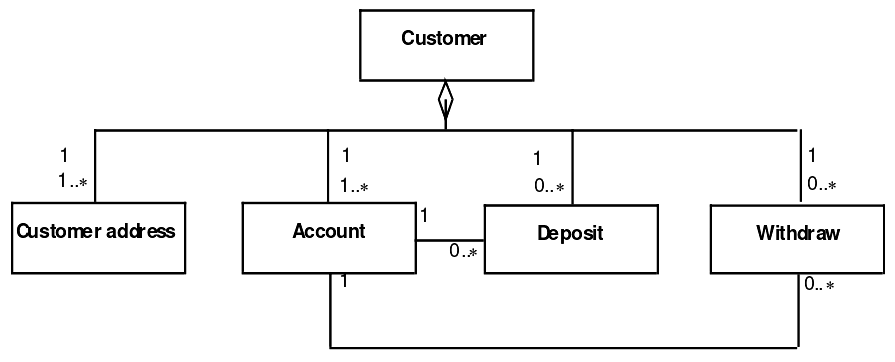
\includegraphics[width=0.7\textwidth]{figures/modelcomponentsolutionb.png}
\end{figure}

\subsection{Restructure classes}
The revised class diagram represents the same information as the statechart diagrams. The class diagram can often be simplified without loss of information; \textbf{generalisation, association, embedded iterations}.

\begin{figure}[H]
    \centering
    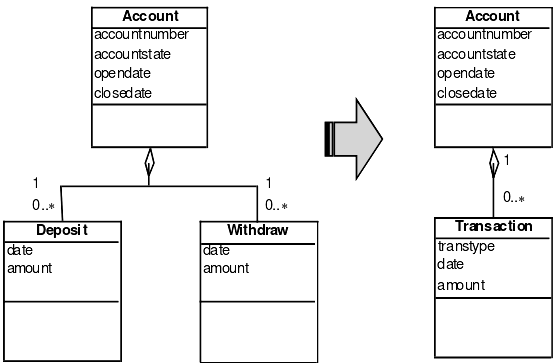
\includegraphics[width=0.7\textwidth]{figures/modelcomponentrestructureclasses.png}
\end{figure}

\begin{itemize}
    \item \textbf{Generalisation}
    \begin{itemize}
        \item Classes with the same attributes will often exist, as there's a need to separate the types of classes. This can be done with an attribute as shown in the transaction example. However, if the operations, \texttt{deposit} and \texttt{withdraw}, differ greatly, the original solution might be better suited.
    \end{itemize}
    \item \textbf{Association}
    \begin{itemize}
        \item When new classes get added, reconsideration of old structures is relevant to see if they can be removed. Notice how the association between Gas station and Customer can be removed as the only important information is whether a Customer filled up, obviously at a Gas station. As the information - \textit{did the customer visit the Gas station} - is apparent from the Filling-class, the original association is redundant and thus removed.
    \end{itemize}
    \item \textbf{Embedded iterations}
    \begin{itemize}
        \item In the figure showing an aggregation of \texttt{Hospitalisation}, \texttt{Treatment}, and \texttt{Discharge} to a \texttt{Person} is a very simple hospital system. This will work, but some important information is missed. A discharge is always preceded by exactly one hospitalisation and a treatment is always connected to exactly one hospitalisation. The simple model cannot hold this information. A better way is to embed this information as shown in the resulting class diagram.
    \end{itemize}
\end{itemize}

The figure below shows unnecessary associations.
\begin{figure}[H]
    \centering
    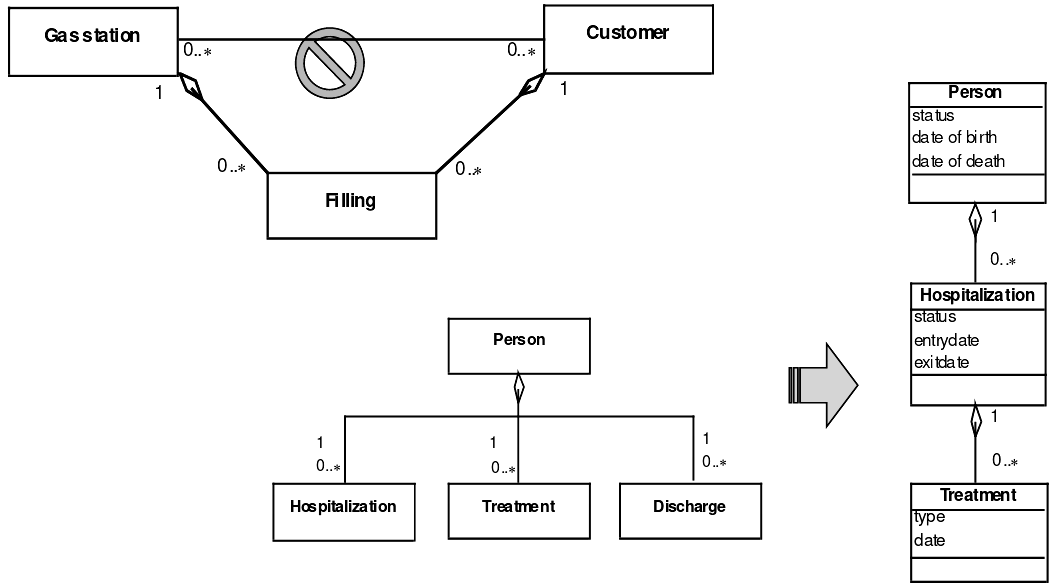
\includegraphics[width=\textwidth]{figures/modelcomponentrestructureclasses2.png}
\end{figure}

\subsection{Summary}
\begin{figure}[H]
    \centering
    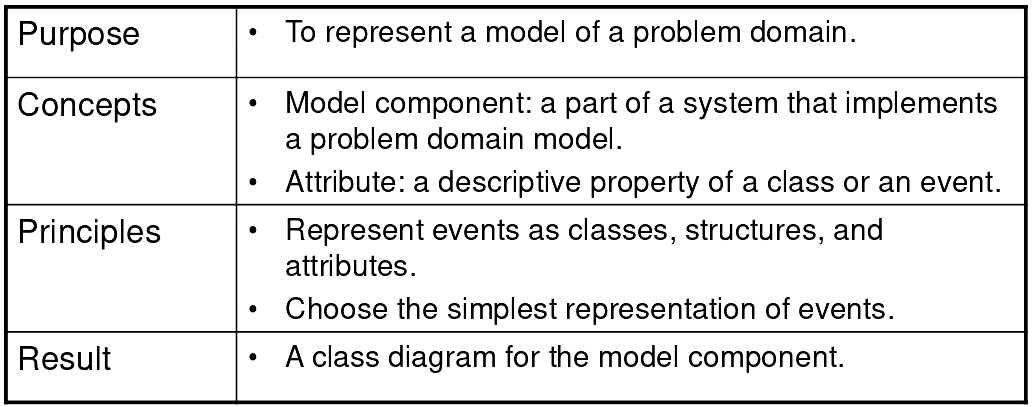
\includegraphics[width=0.7\textwidth]{figures/modelcomponentsummary.png}
\end{figure}

\subsection{Principles}
\subsubsection{Represent events as classes, structures, and attributes}
The class diagram from the analysis activity is revised by systematically representing the objects' events in new classes, structures, and attributes.

\subsubsection{Choose the simplest representation of events}
If a common event is only involved in the iterations, you might have to outline and compare concrete design alternatives.

